\chapter{Introduction}
\label{chap:intro}

Water quenching is a key manufacturing step for aluminium automotive castings.
After heat treatment, the part is submerged in water and cooled rapidly.
The temperature does not drop uniformly.
Thin walls and exposed surfaces lose heat much faster than thick interior regions.
These spatial temperature differences are called thermal gradients.
They drive residual stress and shape distortion in the finished part
\cite{xiao2010,wang2019quenching,mortensen2026}.
In complex three-dimensional (3D) components, different regions cool at
different rates simultaneously.
Predicting these gradients is therefore difficult.

If the temperature prediction is inaccurate, the finished part may fall outside
its dimensional tolerances.
Correcting distortion after manufacture is expensive.
Accurate thermal simulation is therefore central to the design process.

This project addresses the same quenching problem studied by Mortensen
et al.~\cite{mortensen2026}.
Their work used the Finite Element Method (FEM) to model the thermomechanical
behaviour of cast A356 aluminium subframes.
They quantified how quenching causes distortion.
This thesis adopts the same physical setting.
The question asked here is different.
How many FEM solver calls can be replaced by trained neural network predictions
without losing useful accuracy?

FEM is the standard tool for this type of simulation.
It is reliable \cite{wilson1966,mackerle2003,grossmann2024fem}.
In this work it serves as the reference solver.
The solver uses a $0.5\,\mathrm{s}$ internal time step with the
unconditionally stable Crank--Nicolson scheme \cite{grossmann2024fem}.
It records the temperature field every $1.5\,\mathrm{s}$.
Over a 30-second quench, this produces 21 snapshots and 20 prediction
intervals.
FEM is accurate but computationally expensive.
For design studies that repeat the same simulation hundreds of times, the
cost adds up quickly.

To reduce that cost, this thesis combines FEM with Physics-Informed Neural
Networks (PINNs).
A PINN encodes the governing heat equation directly into its training loss.
It produces physically consistent predictions.
Labelled data at every spatial location is not required
\cite{raissi2019,karniadakis2021,zhao2025heattransfer}.
The idea of using neural networks to solve partial differential equations
(PDEs) goes back to Lagaris et al.~\cite{lagaris1998}.
In practice, PINNs are sensitive to the choice of network architecture,
loss weighting, and temporal error accumulation
\cite{wang2021,wang2022ntk,mcclenny2023,guo2023transientheat}.
In transient problems these difficulties grow over time.

The approach taken here divides the 30-second simulation into short prediction
windows.
At the start of each window, FEM provides the current temperature field as a
fixed anchor state.
The PINN then predicts the field over the rest of the window.
The FEM solver always uses its own internal $0.5\,\mathrm{s}$ time step.
Reducing the number of anchor snapshots does not change how FEM runs internally.
Each anchor call is a complete, independent solve from a known state.
The PINN prediction never feeds back into the FEM solver.
Using FEM at selected intervals therefore introduces no additional numerical
instability \cite{grossmann2024fem,meng2020ppinn}.

The skip factor $k \in \{1,2,3,4,5\}$ controls how many FEM anchor snapshots
are used.
At $k=1$, FEM anchors all 20 intervals and there is no saving.
At $k=5$, FEM anchors only 4 of the 20 intervals, an 80\% reduction in solver
calls.
The PINN covers each 7.5-second window between anchors.
This windowed strategy is called Multi-Step Window Prediction (MSWP).

\section{Background}
\label{sec:background}

Water quenching of aluminium alloys produces non-uniform temperature fields.
Different geometric features exchange heat at different rates
\cite{xiao2010,wang2019quenching}.
For simple components this non-uniformity is manageable.
Residual stresses are small and distortions stay within tolerance.
For complex components such as automotive subframes, the situation is more
severe.
Thin rails, enclosed cavities, and varying cross-sections create spatially
heterogeneous cooling patterns \cite{mortensen2026}.
Thermal gradients concentrate near thin features.
The resulting residual stresses can push final dimensions outside engineering
tolerances.
Post-production rework is both time-consuming and costly \cite{xiao2010}.

Accurate simulation of this process requires resolving the spatial temperature
field throughout the component at each time step.
FEM achieves this but at significant computational cost, particularly for
industrial meshes with millions of elements
\cite{grossmann2024fem,mortensen2026}.

\section{Motivation}
\label{sec:motivation}

Mortensen et al.~\cite{mortensen2026} provide a validated FEM framework for
predicting quench-induced distortions in cast A356 aluminium subframes.
They show that rack optimisation can reduce peak distortions from
${\approx}3\,\mathrm{mm}$ to ${\approx}1\,\mathrm{mm}$.
FEM handles complex geometry and time-varying boundary conditions well.
It has been the standard tool for thermal analysis in casting for decades
\cite{wilson1966,mackerle2003,grossmann2024fem}.
The challenge is cost.
A single solve on a fine industrial mesh can take minutes.
Design optimisation studies that repeat the simulation hundreds of times make
this a practical bottleneck.

% [HOCA #7]: "What is a NAS? Never mentioned it before."
% DUZELTME: NAS ilk kullanim oncesinde tanimlandi.
In this thesis, we developed a complementary approach.
We paired PINNs with Neural Architecture Search (NAS).
NAS automates the selection of network width, depth, and activation functions.
The resulting NAS-PINN framework anchors PINN predictions to FEM solutions at
selected time steps.
This reduces FEM solver calls while keeping accuracy within the engineering
tolerances of \cite{mortensen2026}.

\section{Problem Statement}
\label{sec:problem}

% [HOCA #2]: "I don't think we should use this term as it is a specific case
% in the literature." -- "Mortensen-type transient quenching simulations"
% DUZELTME: "Mortensen-type" tamamen kaldirildi.
%
% [HOCA #3]: "Use an illustration to express the idea here. What is NAS-PINN?
% Was never defined."
% DUZELTME: Figure~\ref{fig:pinn_framework} referansi eklendi. NAS-PINN Motivation
% bolumunde tanimlandi.
The proposed FEM-anchored NAS-PINN framework is built around the physical
setting of Mortensen et al.~\cite{mortensen2026}.
It models transient cooling of A356 aluminium from an initial casting
% [HOCA #4]: "Define all variables." -- $T_0
% DUZELTME: T_0 = initial casting temperature, T_w = quench bath temperature olarak tanimlandi.
temperature of $T_0 = 540\,^\circ\mathrm{C}$ to near the quench bath
temperature $T_w = 20\,^\circ\mathrm{C}$ over 30 seconds.
The proprietary industrial mesh and in-house StaMiSim solver data of Mortensen
et al.\ are not publicly available.
This thesis therefore uses the physical parameters and quenching behaviour
reported in that work to construct reproducible surrogate benchmark domains.
These surrogate domains are controlled approximations, not independent
benchmark problems.
They test whether the MSWP approach can reduce FEM solver calls while
preserving the thermal accuracy needed for distortion prediction.

Mortensen et al.\ couple thermal and mechanical FEM at every time step.
This is accurate but expensive.
The mesh has approximately 3 million finite elements across 27--30 coupled
domains.
This thesis proposes a FEM-accelerated hybrid.
FEM is retained as the source of physical truth at periodic anchor points.
NAS-guided PINN predictions replace the majority of time-step solves.
The method is a FEM-call reduction strategy for this class of transient
quenching simulation.
It is not a general-purpose FEM replacement.
The central question is: what is the maximum fraction of FEM solver calls that
the NAS-PINN can replace while keeping temperature errors within the industrial
tolerance required for distortion prediction?

Figure~\ref{fig:timestep_intro} illustrates the three operating modes of the
framework.

\begin{figure}[htbp]
\centering
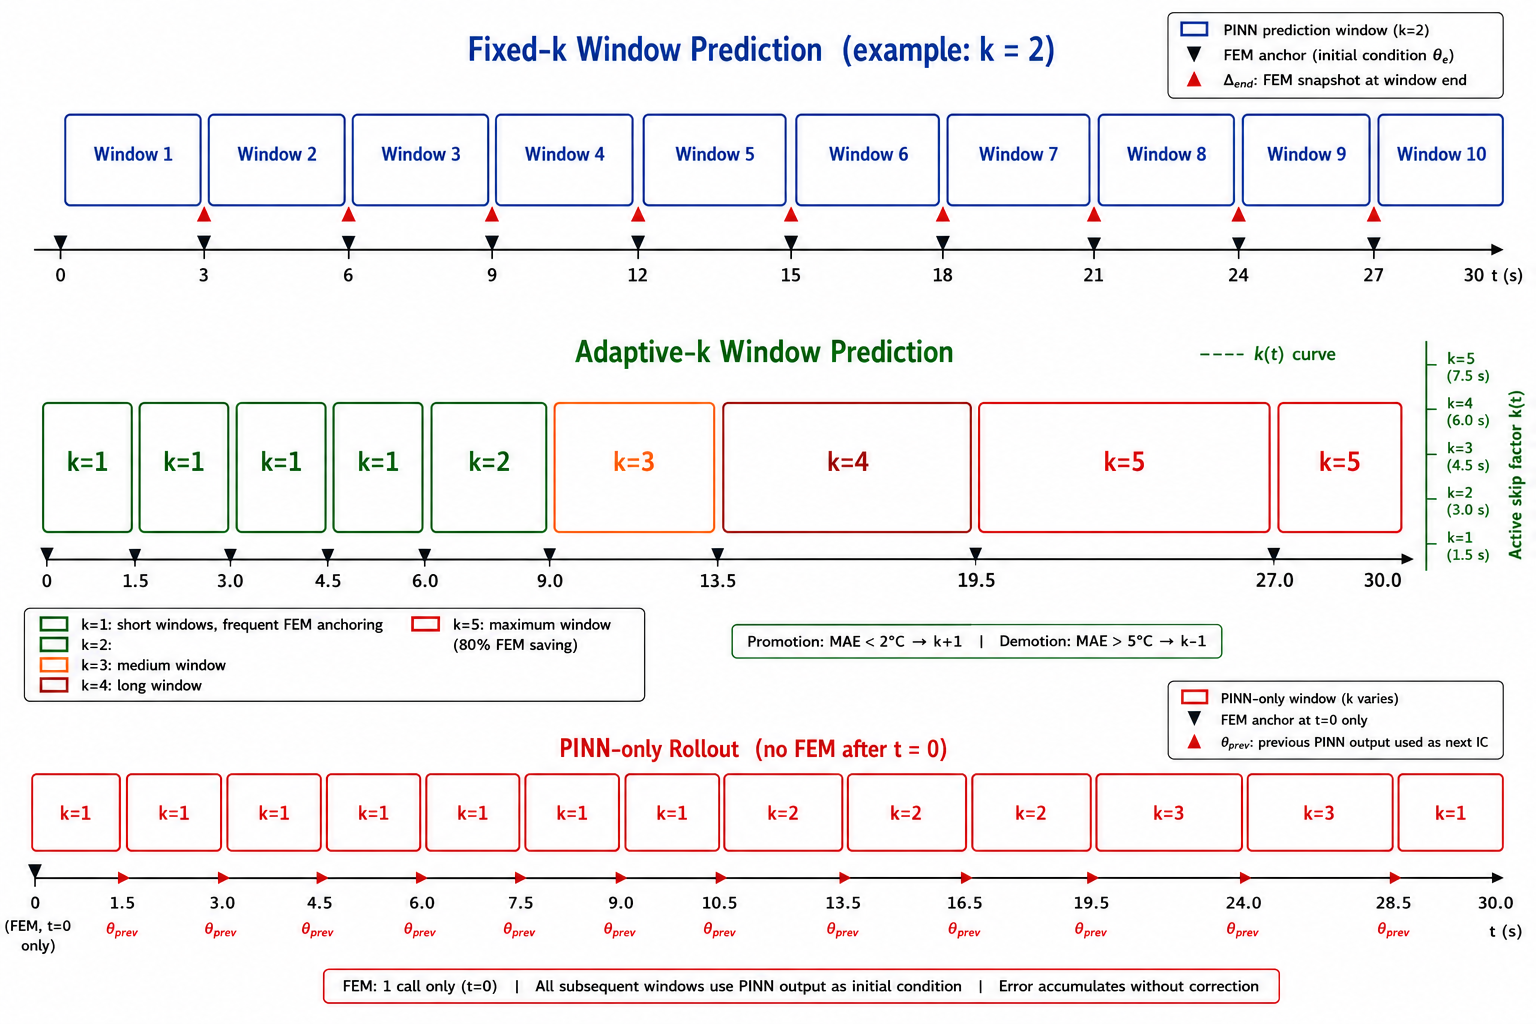
\includegraphics[width=\textwidth]{Figures/fig_mswp_three_modes.png}
\caption{Three operating modes of the MSWP framework.}
\label{fig:timestep_intro}
\end{figure}

In fixed-$k$ mode (top panel), FEM anchors every prediction window.
The PINN predicts each window independently.
Endpoint supervision ($\mathcal{L}_\mathrm{end}$) keeps the prediction aligned
with the next FEM snapshot.
In adaptive-$k$ mode (middle panel), the controller starts at $k=1$.
It promotes to larger $k$ as the field relaxes.
The dashed line shows how $k$ changes over time.
All three NAS architectures reach the same schedule on regular 2D domains.
FEM saving reaches 83--85\%.
In PINN-only mode (bottom panel), FEM is used once at $t=0$.
Each window then uses the previous PINN output as its initial condition.
Errors accumulate without correction.

% [HOCA #1]: "FEM is an iterative method, when we use it at certain intervals,
% wouldn't it make unstable numerically? Justification from the literature needed."
% DUZELTME: Her FEM cagrisinin bagimsiz, tam bir Crank-Nicolson cozumu oldugu
% aciklandi. PINN ciktisi FEM'e geri beslenmez. Kaynak: grossmann2024fem, meng2020ppinn.
This investigation uses the same material and process parameters as Mortensen
et al., with two deliberate simplifications.
% [HOCA #5]: "What are the units here?" -- h=4000 W/(m2K)
% DUZELTME: h tanimlandi: "convective heat transfer coefficient" ve birimi eklendi.
% [HOCA #11]: "Not clear to me, what is h? what is single-phase thermal model?"
% DUZELTME: h yukarida tanimlandi. "Single-phase" = kati hal faz donusumu olmadan termal model olarak aciklandi.
First, rather than the full temperature-dependent boiling curve $h(T)$ of
Mortensen et al., a constant convective heat transfer coefficient
$h$ ($\mathrm{W\,m^{-2}K^{-1}}$) was adopted.
This coefficient measures the heat flux per unit surface area per unit
temperature difference between the metal surface and the quench water.
For 2D benchmark domains $h = 5000\,\mathrm{W\,m^{-2}K^{-1}}$, and for 3D and
surrogate domains $h = 4000\,\mathrm{W\,m^{-2}K^{-1}}$.
Second, no new PINN training algorithm was proposed.
Established techniques were instead combined into a single FEM-anchored
workflow: time-decomposed PINN windows, NAS-driven architecture selection,
Fourier feature embeddings, and self-adaptive loss weighting.
We evaluated the resulting system across ten unique benchmark geometries,
from simple 2D shapes to a 3D Thermal Fin benchmark.

\subsection{Scope}
\label{subsec:scope}

This thesis has three deliberate scope boundaries.
The PINN training algorithm, loss formulation, and stabilisation techniques are
taken from the established literature without modification.
The reference physical problem is taken from Mortensen
et al.~\cite{mortensen2026} to ensure that results connect to a documented
industrial quenching case.
The contribution is a systematic evaluation of when the FEM-anchored hybrid
succeeds and where it fails, across geometries of increasing complexity.
This evaluation helps practitioners judge whether a PINN-based surrogate is
viable for a specific casting geometry.

\section{Contributions}
\label{sec:contributions}

The goal of this research is a computational accelerator for FEM-based
industrial quenching simulations.
The accelerator is a trained NAS-PINN that replaces the majority of FEM solver
calls while staying within the engineering accuracy required for distortion
prediction.
The contributions below constitute the first phase of that programme.
The MSWP framework is built and validated on controlled benchmark geometries
before being applied to the full industrial problem.

We built a reproducible, end-to-end implementation of the FEM-anchored MSWP
framework, combining time-decomposed prediction windows, initial-condition-consistent
network output, NAS-selected architectures, and adaptive skip-factor scheduling.
The code is designed to accept the Mortensen physical parameters and geometry
without structural changes.

The framework was evaluated across ten unique benchmark geometries.
The canonical study covers three 2D domains, four 3D domains, and the Thermal
Fin, a 2D steady-state benchmark from the RBniCS library that we extended to a
full 3D transient quenching scenario.
An additional adaptive-$k$ study covers four 2D domains, together mapping the
accuracy--efficiency trade-off across a wide range of geometric complexity.

Three NAS strategies were compared: Bayesian/TPE, NSGA-II, and NSGA-III.
This comparison provides empirical guidance on which architecture type to deploy
on complex casting geometries.

We also characterised the failure modes of PINN-only rollouts.
On geometries with reentrant edges, thin features, or enclosed cavities,
PINN-only predictions reached errors three to eighteen times higher than the
FEM-anchored hybrid, establishing that FEM anchoring is a required component
of the workflow.

The NAS-PINN was benchmarked against temporal linear interpolation between FEM
snapshots.
On smooth geometries, interpolation achieves lower $L_2$ field error, but on
geometries with enclosed cavities or reentrant corners it fails to reproduce
the spatial heterogeneity.
The NAS-PINN retains accuracy in these complex cases.

Finally, we evaluated the adaptive-$k$ strategy on four 2D domains: Square,
Circle, L-Shape, and Flower.
All architectures achieved 83--85\% FEM saving with mean-window MAE below
$2.5\,^\circ\mathrm{C}$, confirming that adaptive skip-factor scheduling
outperforms fixed-$k$ on these geometrically regular domains.

\section{Thesis Structure}

The remainder of the thesis is structured as follows.
Chapter~\ref{chap:theory} covers heat transfer, FEM, PINNs, and NAS.
Chapter~\ref{chap:method} describes the prediction framework, the network
formulation, training setup, and benchmark domains.
Chapter~\ref{chap:results} presents the results.
Chapter~\ref{chap:discussion} explains what the results mean and where the
method holds up.
Chapter~\ref{chap:conclusion} summarises the findings and outlines the next
steps.
